\chapter{Linear Mapping}
\begin{definition}
Let us consider 2 vector spaces $V$ and $W$. A function $\Lm:V\to W$ is called a linear mapping, if:
\begin{enumerate}
\item For any $\vv\in V$ and $\vv'\in V$, $\Lm(\vv+\vv') = \Lm(\vv)+\Lm(\vv')$
\item For any $\vv\in V$ and any scalar $\alpha$, $\Lm (\alpha\vv) = \alpha\cdot\Lm(\vv)$
\end{enumerate}
\end{definition}
\begin{example}
Let us consider matrix $A\in\R^{n,m}$. We can define linear mapping $\Lm_A$ as follows:
\[
\Lm_A(\vv) = A\vv\hspace{5mm}\Lm_A:\R^m\to\R^n
\]	
Is $\Lm_A$ a linear mapping? Yes!
\begin{proof}
\begin{enumerate}
\item $\forall \vv,\vv'\in\R^m$, we have: $$\Lm_A(\vv+\vv') = A(\vv+\vv') = A\vv+A\vv' = \Lm_A(\vv) + \Lm_A(\vv')$$
\item $\forall\vv\in\R^m,\forall\alpha$ ($\alpha$ is scalar), we have: $$\Lm_A(\alpha\vv) = A(\alpha\vv) = \alpha\cdot A\vv = \alpha \Lm_A(\vv)$$
\end{enumerate}
\end{proof}

\end{example}
Let us consider matrix $A\in\R^{n,m}$, $A:\R^m\to\R^n$. Let us consider vector $\vv\in\R^m$
.
\[
A\vv = \underbrace{v_1\cdot\colvec{3}{a_{11}}{\vdots}{a_{n1}} + v_2\cdot\colvec{3}{a_{12}}{\vdots}{a_{n2}}+ ... + v_m\cdot\colvec{3}{a_{1m}}{\vdots}{a_{nm}}}_{\text{Linear combination of columns of $A$}}
\]

\begin{center}
\begin{tikzpicture}[scale=1.2]

\draw[] (0,0) --(2,0) --(2,3) -- (0,3)--cycle;
\draw (2,3) node[anchor=north east]{$\R^m$};

\draw[] (5,0) --(7,0) --(7,3) -- (5,3)--cycle;
\draw (7,3) node[anchor=north east]{$\R^n$};

\draw[fill=black] (1,2) circle (0.03);
\draw[fill=black] (0.8,0.8) circle (0.03);
\draw (0.9,1.5) node[anchor=east]{0};
\draw[fill=black] (0.9,1.5) circle (0.03);
\draw (1,2) node[anchor=south]{$\vv$};
\draw[fill=black] (1.7,1.5) circle (0.03);

\draw[rotate=315,shift={(-2.75,3.75)}] (5.5,1) --(6.5,1) --(6.5,2.2) -- (5.5,2.2)--cycle;
\draw[->](5.9,1.4)--(6.3,1.4);
\draw[->](5.9,1.4)--(6.15,1.7);

\draw [->] (1,2) parabola bend (3.6,2.5) (6.2,2);
\draw [->] (0.8,0.8) parabola bend (3.4,0.6) (6,1);
\draw [->] (1.7,1.5) parabola bend (3.6,1.8) (5.7,1.5);
\draw (6.8,1.85) node[anchor=north east]{\tiny{$A\ul{v}$}};
\draw[<-] (6.2,1) -- (6.2,-0.5) node [anchor=north,xshift=-30]{span of columns of $A$};
\end{tikzpicture}
\end{center}

\begin{example}
\begin{enumerate}
\item 
\[
A\in\R^{2,2} = \begin{pmatrix}
1 & 3\\
1 & -1
\end{pmatrix}
\]
\begin{center}
\begin{tikzpicture}[scale=0.45]
\draw[->](-4,0)--(4,0) node[anchor=west]{$x_1$};
\draw[->](0,-4)--(0,4)node[anchor=south]{$x_2$};
\draw[fill=black] (1,2) circle (0.04);
\draw[fill=black] (1,-1) circle (0.04);

\newcommand{\offsetDrawing}{12}
\draw [->] (1,2) parabola bend (7,3) (1+\offsetDrawing,2);
\draw [->] (1,-1) parabola bend (7,-2) (1+\offsetDrawing,-1);




\draw[->](-4+\offsetDrawing,0)--(4+\offsetDrawing,0) node[anchor=west]{$x_1$};
\draw[->](0+\offsetDrawing,-4)--(0+\offsetDrawing,4)node[anchor=south]{$x_2$};

\draw[->,thick](0+\offsetDrawing,0)--(1+\offsetDrawing,1) node[anchor=west]{Col. 1 of $A$};
\draw[->,thick](0+\offsetDrawing,0)--(3+\offsetDrawing,-1) node[anchor=west]{Col. 2 of $A$};

\draw[] (-4,4) node{$\R^2$};
\draw[] (4+\offsetDrawing,4) node{$\R^2$};
\end{tikzpicture}
\end{center}
\item \[
A = \begin{pmatrix}
1 & 3\\
2 & 6
\end{pmatrix}
\]
\begin{center}
\begin{tikzpicture}[scale=0.45]
\draw[->](-4,0)--(4,0) node[anchor=west]{$x_1$};
\draw[->](0,-4)--(0,4)node[anchor=south]{$x_2$};
\draw[fill=black] (0.8,1.2) circle (0.04);
\draw[fill=black] (1,-1) circle (0.04);
\draw[fill=black] (-1,2) circle (0.04);
\newcommand{\offsetDrawing}{12}
\draw [->] (0.8,1.2) parabola bend (5.5,2) (-0.25+\offsetDrawing,-0.5);
\draw [->] (1,-1) parabola bend (6.25,-1.5) (-0.5+\offsetDrawing,-1);
\draw [->] (-1,2) parabola bend (5,3) (0.95+\offsetDrawing,2);



\draw[->](-4+\offsetDrawing,0)--(4+\offsetDrawing,0) node[anchor=west]{$x_1$};
\draw[->](0+\offsetDrawing,-4)--(0+\offsetDrawing,4)node[anchor=south]{$x_2$};

\draw[->,thick](0+\offsetDrawing,0)--(0.5+\offsetDrawing,1) ;
\draw[->,thick](0+\offsetDrawing,0)--(1.5+\offsetDrawing,3);
\draw[](-1.5+\offsetDrawing,-3)--(1.75+\offsetDrawing,3.5);

\draw[] (-4,4) node{$\R^2$};
\draw[] (4+\offsetDrawing,4) node{$\R^2$};
\draw[] (3.4+\offsetDrawing,3.2) node{$\leftarrow$ span of cols. of $A$};
\end{tikzpicture}
\end{center}

\end{enumerate}
	
\end{example}

\begin{note}
In order for solution of $A\ul{x} = \ul{b}$ to exist, $\ul{b}$ should belong to a span of columns of matrix $A$.	
\end{note}

\begin{definition}
The span of columns of matrix $A \in \R^{n, m}$ is called a column space of $A$, denoted by $C(A)$, where $C(A)\subset R^n$.
\end{definition}
\begin{definition}
Let us consider matrix $A\in\R^{n,m}, A:\R^m\to \R^n$. The null space of $A$ is defined as 
\[
N(A) = \left\{ \vv\in\R^m\mid A\vv = \ul{0}\right\}, N(A)\subset\R^m
\]
\begin{center}
\begin{tikzpicture}[scale=0.75]

\draw[] (0,0) --(3,0) --(3,5) -- (0,5)--cycle;
\draw (3,5) node[anchor=north east]{$\R^m$};

\draw[] (7,0) --(10,0) --(10,5) -- (7,5)--cycle;
\draw (10,5) node[anchor=north east]{$\R^n$};

\draw[rotate=-45,xshift=-55] (0.5,2) --(0.5,4) --(2,4) -- (2,2)--cycle;
\draw[->](1.65,2.65) -- (1.65,3.10);
\draw[->](1.65,2.65) -- (2.10,2.65);

\draw(0.5,2.5) node[anchor=west]{\tiny{$N(A)$}};
\draw(2.75,2.9) node[anchor=east]{\tiny{$\vv$}};
\draw[fill=black](2.55,2.7) circle (0.04);
\draw[fill=black](1.5,2) circle (0.04);

\draw[->](8.5,2.5) -- (8.5,3.5);
\draw[->](8.5,2.5) -- (9.5,2.5);

\draw [->] (2.55,2.7) parabola bend (5.5,3.3) (8.5,2.5);
\draw [->] (1.5,2) parabola bend (5,1.5) (8.5,2.5);

\end{tikzpicture}
\end{center}

\end{definition}
\begin{example}
\[
A = \begin{pmatrix}
1 & 3 \\
2 & 6
\end{pmatrix}
\]	
What is $N(A)$? We should find all solutions of $A\ul{x} = \ul{0}$, this will give us $N(A)$.
\[
\begin{cases}
x_1 + 3x_2 = 0\\
2x_1+6x_2 = 0
\end{cases} \to\begin{cases}
x_1+3x_2=0\\
0 = 0
\end{cases}\to\begin{cases}
x_1=-3x_2\\
0 = 0
\end{cases}\]
The nullspace of this matrix will be a line formed by a linear combination of the vector $\colvec{2}{-3}{1}$ ($\alpha\cdot\colvec{2}{-3}{1}$, for all possible $\alpha$), or in other words it will be the $span(\colvec{2}{-3}{1})$.
\[
x_1 = -3x_2 = -3\alpha,x_2=\alpha\to\alpha\colvec{2}{-3}{1},\alpha\colvec{2}{-6}{2}
\]

\begin{center}
\begin{tikzpicture}[scale=0.45]
\draw[->](-4,0)--(4,0) node[anchor=west]{$x_1$};
\draw[->](0,-4)--(0,4)node[anchor=south]{$x_2$};

\newcommand{\offsetDrawing}{12}
\draw [->] (-1.7,1.7) parabola bend (5.15,3) (-0.05+\offsetDrawing,0.05);
\draw [->] (1.2,-1.2) parabola bend (5.9,-2) (-0.05+\offsetDrawing,-0.05);

\draw[fill=black] (0+\offsetDrawing,0) circle (0.05);


\draw[->](-4+\offsetDrawing,0)--(4+\offsetDrawing,0) node[anchor=west]{$x_1$};
\draw[->](0+\offsetDrawing,-4)--(0+\offsetDrawing,4)node[anchor=south]{$x_2$};
\draw(-3,3) -- (3,-3);
\draw[thick,->](0,0) -- (1,-1);

\draw[] (-4,4) node{$\R^2$};
\draw[] (4+\offsetDrawing,4) node{$\R^2$};
\draw[] (3,-3) node[anchor=west]{$\leftarrow N(A)$};
\end{tikzpicture}
\end{center}
\end{example}
\begin{theorem}
The nullspace, $N(A)$, of $A\in\R^{n,m}$ is a subspace of $\R^m$.
\end{theorem}
\begin{proof}
Let us assume that $\ul{x},\ul{x}'\in N(A)$ and $\alpha$ is arbitrarily scalar. 
\begin{enumerate}
\item $A(\ul{x}+\ul{x}') = A\ul{x}+A\ul{x}' = \ul{0} + \ul{0} = \ul{0} \Rightarrow (\ul{x}+\ul{x}')\in N(A)$\\
\item $A(\alpha\ul{x}) = \alpha (A\ul{x}) = \alpha\cdot \ul{0} = \ul{0}\Rightarrow \alpha\ul{x}\in N(A)$
\end{enumerate}
\end{proof}

\begin{theorem}
The column space, $C(A)$, of $A\in\R^{n,m}$ is a subspace of $\R^n$.
\end{theorem}

\begin{definition}
The row space of matrix $A \in R^{n, m}$ is a span of rows of $A$. Clearly, $R(A)=C(A^T)$ and $R(A)\subset \R^m$.
\end{definition}
\begin{definition}
The left nullspace of $A$ is defined as $N(A^T)$. $N(A^T)\subset\R^n$.
\end{definition}
\begin{theorem}
$R(A)$ is a subspace of $\R^m$
\end{theorem}
\begin{proof}
Same as for the proof that $C(A)$ is a subspace of $\R^{n}$, but for $A^T$
\end{proof}
\begin{theorem}
$N(A^T)$ is a subspace of $\R^n$
\end{theorem}
\begin{proof}
Same as for $N(A)$ but replace $A$ with $A^T$
\end{proof}

\begin{theorem}
$R(A)$ and $N(A)$ are orthogonal subspaces in $\R^m$ for $A\in\R^{n,m}$
\end{theorem}

\begin{proof}
Let us consider $\forall \ul{x}\in N(A), A\ul{x} = \ul{0}$
\[
A\ul{x} = \colvec{3}{-\text{ row 1 of }A\to}{\vdots}{-\text{ row $n$ of }A\to}\cdot \colvec{3}{\mid}{x}{\downarrow} = \colvec{3}{<\text{ row 1 of }A,\ul{x}>}{\vdots}{{<\text{ row $n$ of }A,\ul{x}>}} \mathop=\limits^{\ul{x}\in N(A)}\colvec{3}{0}{\vdots}{0}
\]
$\ul{x}$ is orthogonal to every row of $A$. $\ul{x}$ is orthogonal to every linear combination of rows of $A$. $\ul{x}$ is orthogonal to $R(A)$. In fact, what we just showed is that $N(A)$ \& $R(A)$ are orthogonal complements. 
\end{proof}

\begin{theorem}
$N(A^T)$ \& $C(A) = R(A^T)$ are orthogonal complements in $\R^n$
\end{theorem}

$A\in\R^{n,m}:\R^m\to\R^n$. Row rank of $A = \rank(A) = \dim\left( R(A) \right) =  \dim\left( C(A) \right)$
\begin{align*}
N(A) &:A\ul{x} = \ul{0}\hspace{5mm}\forall x\in\R^m\\
C(A) &: A\ul{v} = \text{ Linear combinations of columns of $A$}\\
&\hspace{7.5mm}= v_1\cdot\text{col 1 of $A$}+\dots+v_n\cdot\text{col $n$ of $A$}\in \R^n
\end{align*}
\begin{theorem}
$N(A)$ is an orthogonal complement of $R(A)$ in $\R^m$,
\[
\dim N(A)+\underbrace{\dim R(A)}_{=\rank(A)}=m
\]
\end{theorem}

\begin{theorem}
$N(A^T)$ is an orthogonal complement of $R(A^T) = C(A)$ in $\R^n$,
\[
\dim N(A^T)+\underbrace{\dim C(A)}_{=\rank(A)}=n
\]
\end{theorem}
\\

Let us consider $A\in\R^{n,m},A:\R^m\to\R^n,\rank(A)=r$
\begin{center}
{\begin{tikzpicture}[scale=0.6, every node/.style={transform shape}]
\path[use as bounding box] (-2,-8) rectangle (17,4);
\draw[rotate=-45](0,0)--(0,5)--(3,5)--(3,0)--cycle;
\draw[rotate=45,shift={(-3,-8)}](0,0)--(0,5)--(3,5)--(3,0)--cycle;
\draw[rotate=-45,shift={(3,0)}] (0.3,0) -- (0.3,0.3) -- (0,0.3);
\draw[rotate=-45,shift={(2.25,-0.75)},dashed] (2,0) -- (2,2) -- (0,2);
\draw[fill=black](3.85,-2.15) circle (0.075);
\draw[fill=black](3.85,-2.15) node[anchor=west]{$x_r+x_n$};

\draw (0,-2.15) node {2 orthogonal spaces};
\draw[->](0,-2)--(0.75,-1.25);
\draw[->](0,-2.4)--(0.75,-3.2);
\draw[->](-0,15)--(20,15);
\draw (3.5,-7) node {$N(A)$};
\draw (3.5,2.8) node {$R(A)$};
\draw (3,1.5) node {$\dim R(A) = r$};
\draw (3,-5.5) node {$\dim N(A) = m-r$};
\draw (2.5,-3.8) node {$\ul{x}_n$};
\draw (2.5,-0.5) node {$\ul{x}_r$};
\draw (0,3) node {$\R^n$};

\begin{scope}[xshift=300]
\draw[rotate=-45](0,0)--(0,5)--(3,5)--(3,0)--cycle;
\draw[rotate=45,shift={(-3,-8)}](0,0)--(0,5)--(3,5)--(3,0)--cycle;
\draw[rotate=-45,shift={(3,0)}] (0.3,0) -- (0.3,0.3) -- (0,0.3);
\draw (3.5,-7) node {$N(A^T)$};
\draw (3.5,2.8) node {$C(A)$};
\draw (3,1.5) node {$\dim C(A) = r$};
\draw (3.5,-5.5) node {$\dim N(A^T) = n-r$};
\draw (2.5,-0.5) node {$A\ul{x}_r = \ul{b}$};
\draw (0,3) node {$\R^n$};
\end{scope}

\draw[->](2.75,-0.5) --(12,-0.5);
\draw[->] (5.2,-2.15) -- (12,-0.7);
\draw[] (7.8,-0.9) node {$A(x_r+x_n)=Ax_r+Ax_n = Ax_r = b$};
\draw[->] (2.75,-3.8) -- (12.3,-2.15);
\end{tikzpicture}}
\end{center}

\begin{lemma}
For any vector $\ul{b}$ in $C(A)$, there exists one and only one vector $\ul{x}_r\in R(A)$ such that $A\ul{x}_r=b$
\end{lemma}

\begin{proof}
Let us assume that $\ul{x}_r$ and $\ul{x}_r'$ are in the row space, $R(A)$. Let us assume that $A\ul{x}_r = A\ul{x}_r'$. We have
\[
\ul{x}_r \in R(A) - \ul{x}_r' \in R(A) \in R(A)
\]
But we also have 
\[
A\ul{x}_r -A\ul{x}_r' = \underbrace{A(\ul{x}_r-\ul{x}_r' }_{\in N(A)} = \ul{0} 
\]
It means that $(\ul{x}_r-\ul{x}_r' )$ is in $R(A)$ and $N(A)$, but they are orthogonal subspaces, therefore 
\[
\ul{x}_r-\ul{x}_r' =\ul{0}\Rightarrow \ul{x}_r=\ul{x}_r' 
\]
\end{proof}
\begin{example}
Let us consider
\[
A = \begin{pmatrix}
1 & -2 \\
-1 & 2
\end{pmatrix}\in\R^{2,2}
\]	
\begin{center}
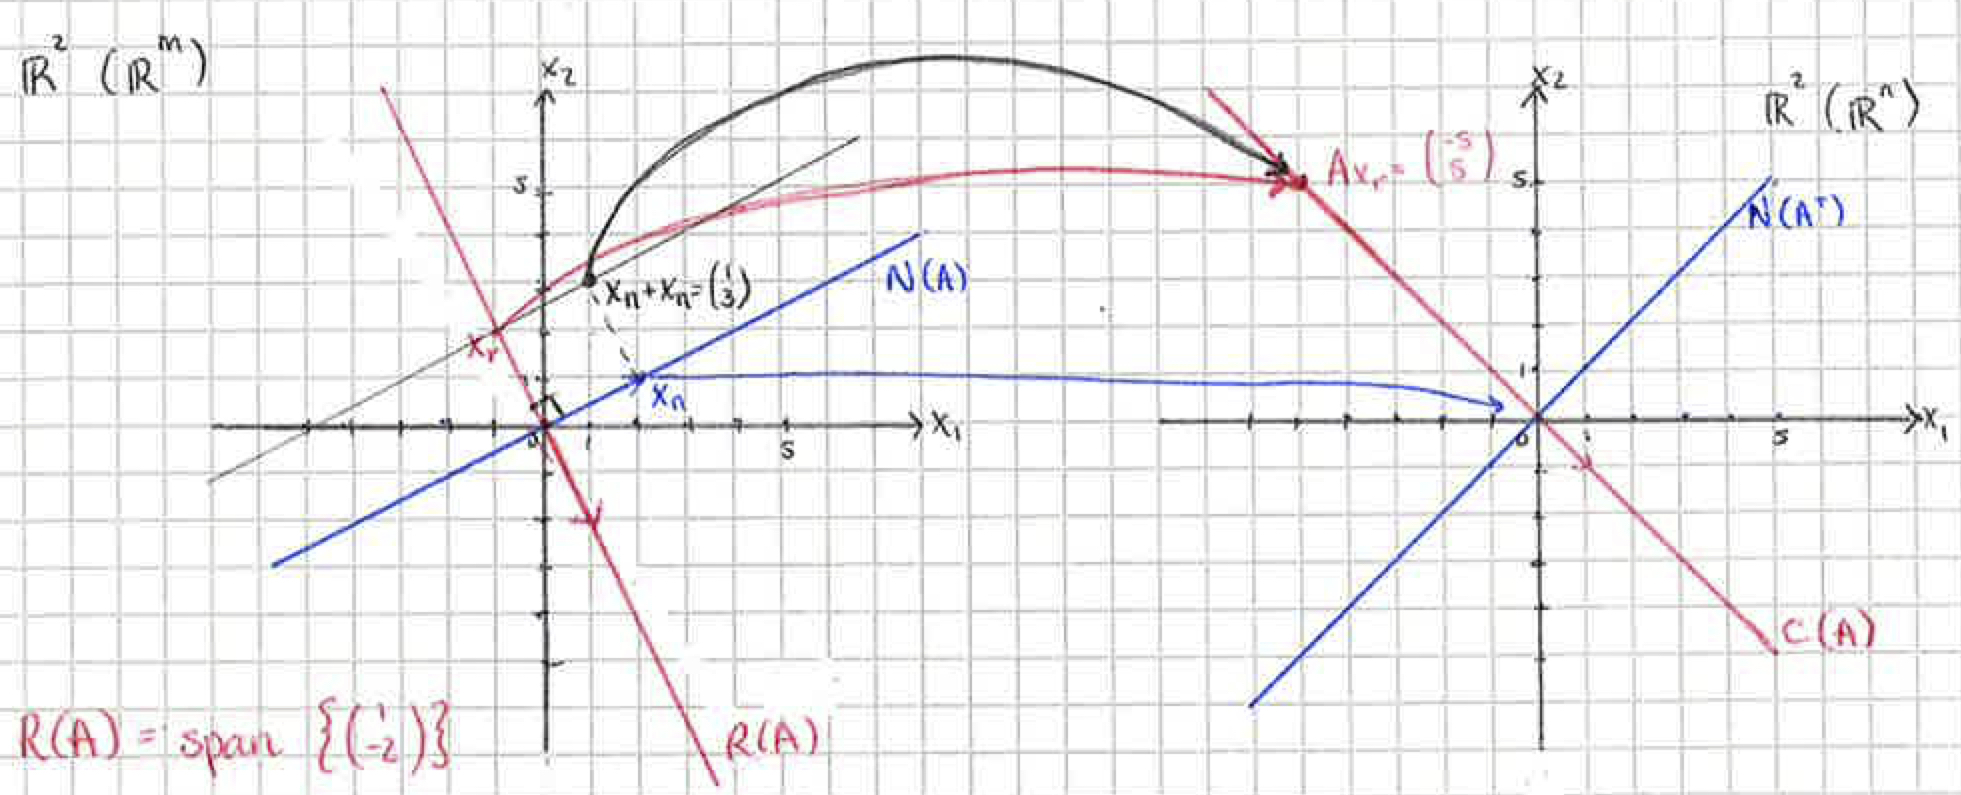
\includegraphics[scale=0.17]{Other/imageToSubstitute}
\end{center}

\end{example}
Row space: $\rank A = 1\Rightarrow \dim R(A)=1$
\[
R(A) = \text{span}\left\{ \colvec{2}{1}{-2},\colvec{2}{-1}{2}\right\} = \text{span} \left\{ \colvec{2}{1}{-2}\right\}
\]
Null space: $\dim N(A) = 2-1 = 1$
\[
A\ul{x} = 0\Rightarrow \begin{cases}
x_1-2x_2 = 0\\
-x_1+2x_2 = 0\\
\end{cases} \Rightarrow\begin{cases}
x_1-2x_2 = 0\\
0 = 0\\
\end{cases}\Rightarrow x_1 = 2x_2\text{ (Line)}
\]
Column space: $\dim C(A) = \dim R(A) = \perp$
\[
C(A) = \text{span}\left\{ \colvec{2}{1}{-1},\colvec{2}{-2}{2}\right\} = \text{span}\left\{\colvec{2}{1}{-1}\right\}
\]
Left Null space: $\dim N(A^T) = 2-1=1$. Consider 
\begin{align*}
\ul{x}_r &= \colvec{2}{-1}{2}\Rightarrow A\ul{x}_r =\begin{pmatrix}
1 & -2\\
-1 & 2	
\end{pmatrix}\colvec{2}{-1}{2} = \colvec{2}{-5}{5}\\
\ul{x}_n &= \colvec{2}{2}{1}\Rightarrow A\ul{x}_n =\begin{pmatrix}
1 & -2\\
-1 & 2	
\end{pmatrix}\colvec{2}{2}{1} = \colvec{2}{0}{0}
\end{align*}

\section{Orthogonal Basis and Gram-Schmidt process}
\begin{definition}
Vectors $\ul{q}_1,\dots,\ul{q}_m$ are orthogonal if:
\[
\langle \ul{q}_i,\ul{q}_j\rangle = \ul{q}_i^T\ul{q}_j=0\hspace{5mm}\text{if }i\not=j
\]
\end{definition}

\begin{definition}
Vectors $\ul{q}_1,\dots,\ul{q}_m$ are orthonormal if:
\[
\langle \ul{q}_i,\ul{q}_j\rangle = \ul{q}_i^T\ul{q}_j=\begin{cases}
0 & \text{if }i\not=j\\
1 & \text{if }i=j\\
\end{cases}
\]
\end{definition}
If the columns of the matrix are orthonormal vectors, then this matrix is usually denoted by $Q$, In this case, we have $Q^TQ=I$. If $Q$ is not a square matrix then $QQ^T$ is not necessarily $I$.

\begin{definition}
A square matrix is called orthogonal (if its columns are orthonormal vectors) if $Q^TQ=I$. In this case, since it is a square matrix, $QQ^T=I$
\end{definition}

\subsection{Projection on the line}
Let us assume that we have a line given by vector $\ul{a}=\colvec{3}{a_1}{\vdots}{a_n}\in\R^n$ and vector $\ul{b}\in\R^n$. We want to find vector $\ul{p}$ belonging to the line, closest to vector $\ul{b}$. In other words, we are looking for $\ul{p}$ which is orthogonal projection of $\ul{b}$ onto the line given by $\ul{a}$
\begin{center}
\begin{tikzpicture}[scale=0.75]
\draw[->] (-1,0) -- (5,0);
\draw[->] (0,-1) -- (0,5);
\draw[->,thick] (0,0) -- (2,4);
\draw[->,thick] (0,0) -- (4,3);
\draw[] (1.5,3) -- (2.9,2.17);
\draw (0.8,2) node {$\ul{a}$};
\draw (2.5,1.5) node {$\ul{b}$};
\draw (2.2,2.9) node {$\ul{e}$};
\draw[yshift=73,xshift=35,scale=0.1] (2.1,3) -- (3.5,2.17);
\draw[yshift=73,xshift=53.5,scale=0.1,rotate=90] (2.1,3) -- (3.5,2.17);
\end{tikzpicture}
\end{center}

$\ul{p}$ is proportional to $\ul{a}$, $\ul{p} = \hat{x}\ul{a}$, where $\hat{x}$ is some scalar. Let us define vector $\ul{e} = \ul{b}-\ul{p} = \ul{b} -\hat{x}\ul{a}$ (error vector). $\ul{e}$ is orthogonal to the line, therefore 
\begin{align*}
\langle\ul{a},\ul{e} \rangle &= 0\\
\langle\ul{a},\ul{e} \rangle &=\ul{a}^T(\ul(b)-\hat{x}\ul{a}) = \ul{a}^T\ul{b}-\hat{x}\ul{a}^T\ul{a} = 0\\
\Rightarrow \hat{x} &= \frac{\ul{a}^T\ul{b}}{\ul{a}^T\ul{a}}\\
\Rightarrow \ul{p} &= \hat{x}\ul{a} = \ul{a}\hat{x} = \ul{a}\frac{\ul{a}^T\ul{b}}{\ul{a}^T\ul{a}} = \underbrace{\frac{\ul{a}\ul{a}^T}{\ul{a}^T\ul{a}}}_{P\in\R^{n,n}\text{ (projection matrix)}}\cdot\ul{b}
\end{align*}
\begin{example}
Let us consider $\ul{a}=\colvec{3}{1}{2}{2}	\in\R^3$
\[
P = \frac{\ul{a}^T\ul{b}}{\ul{a}^T\ul{a}} = \langle \colvec{3}{1}{2}{2},\begin{pmatrix}
1 & 2 & 2
\end{pmatrix}\rangle\cdot\frac{1}{9} = \frac{1}{9}\cdot\begin{pmatrix}
1 & 2 & 2\\
2 & 4 & 4\\
2 & 4 & 4
\end{pmatrix}
\]
Let us take
\[
\ul{b} = \colvec{3}{1}{1}{1},\ul{p}=P\ul{b} = \frac{1}{9}\begin{pmatrix}
1 & 2 & 2\\
2 & 4 & 4\\
2 & 4 & 4
\end{pmatrix}\colvec{3}{1}{1}{1} = \frac{1}{9}\colvec{3}{5}{10}{10}
\]
\end{example}
\begin{note}
$\ul{p}^2 = \ul{p}$
\end{note}
\begin{note}
$(I-P)-$ projection onto subspace orthogonal to the line given by $\ul{a}$
\end{note}

\section{Gram-Schmidt process}
Given linear independent vectors $\ul{a},\ul{b},\ul{c},\dots$ we first find orthogonal vectors $\ul{a}',\ul{b}',\ul{c}',\dots$ which span the same subspace as $\ul{a},\ul{b},\ul{c},\dots$ and then we normalise them,
\[
\ul{q}_1 = \frac{\ul{a}'}{\norm{\ul{a}'}},\ul{q}_2 = \frac{\ul{b}'}{\norm{\ul{b}'}},\ul{q}_3 = \frac{\ul{c}'}{\norm{\ul{c}'}},\dots
\]
So, Gram-Schmidt process allows us to construct an orthogonal basis of span$\{\ul{a},\ul{b},\ul{c},\dots\}\in$\todo{Cannot read, page 48 middle}
\begin{enumerate}
\item Choose $\ul{a}' = \ul{a}$
\item It is likely that $\ul{b}$ is not orthogonal to $\ul{a}'$, so we need to subtract its projection on the line defined by $\ul{a}'$
\[
\ul{b}' = \ul{b}-\frac{\ul{a}^T\ul{b}}{\ul{a}^T\ul{a}}\ul{a}'
\]
\item $\ul{c}'$ is likely not orthogonal to $\ul{a}'$ and $\ul{b}'$. Again, subtract its projections
\[
\ul{c}' = \ul{c}-\frac{\ul{a}^T\ul{c}}{\ul{a}^T\ul{a}}\ul{a}'-\frac{\ul{b'}^T\ul{c}}{\ul{b'}^T\ul{b'}}\ul{b}'
\]
and so on. Finally, normalise $\ul{q}_1,\ul{q}_2,\ul{q}_3,\dots$
\end{enumerate}
\begin{example}
With 
\[
\ul{a} = \colvec{3}{1}{-1}{0},\ul{b} = \colvec{3}{2}{0}{-2},\ul{c} = \colvec{3}{3}{-3}{3}
\]	
find $\ul{a}',\ul{b}',\ul{c}',\ul{q}_1,\ul{q}_2,\ul{q}_3$
\begin{enumerate}
\item \[
\ul{a}' = \ul{a} = \colvec{3}{1}{-1}{0}
\]
\item \[
\ul{b'} = \ul{b} -\frac{\ul{a'}^T\ul{b}}{\ul{a'}^T\ul{a'}}\ul{a}' = \colvec{3}{2}{0}{-2} - \frac{\langle \colvec{3}{1}{-1}{0}, \colvec{3}{2}{0}{-2}\rangle}{\colvec{3}{1}{-1}{0},\colvec{3}{1}{-1}{0}} = \colvec{3}{1}{1}{2}
\]
\item \[
\ul{c}' = \ul{c}-\frac{\ul{a}^T\ul{c}}{\ul{a}^T\ul{a}}\ul{a}'-\frac{\ul{b'}^T\ul{c}}{\ul{b'}^T\ul{b'}}\ul{b}' = \colvec{3}{1}{1}{1}
\]
\[
\langle \ul{a}',\ul{c}'\rangle = 0, \langle \ul{b}',\ul{c}'\rangle = 0
\]
Finally normalise:
\[
\ul{q}_1 = \frac{\ul{a}'}{\norm{\ul{a}'}} = \frac{1}{\sqrt{2}}\colvec{3}{1}{-1}{0},\ul{q}_2 = \frac{\ul{b}'}{\norm{\ul{b}'}} = \frac{1}{\sqrt{6}}\colvec{3}{1}{1}{-2},\ul{q}_3 = \frac{\ul{c}'}{\norm{\ul{c}'}} = \frac{1}{\sqrt{3}}\colvec{3}{1}{1}{1}
\]
\end{enumerate}
\end{example}
\section{Projection onto subspace}
Assume we have linearly independent vectors $a_1,\dots,a_m\in\R^n$. We want to project vector $\ul{b}\in\R^n$ onto subspace spanned by $a_1,\dots,a_m$. Subspace consists of all linear combinations
\[
x_1a_1+\dots+x_ma_m =\underbrace{\begin{pmatrix}
\mid & {} & \mid\\
a_1 & \dots & a_m\\
\downarrow & {} & \downarrow 
\end{pmatrix}}_{A\in\R^{n,m}}\cdot \underbrace{\hat{x}}_{\in\R^m}
\]
We are looking for the projection $\ul{p}$ of $\ul{b}$ onto his subspace. We can define $\ul{e}=\ul{b}-\ul{p},\ul{e}$ should be orthogonal to all $a_1,\dots,a_m$
\[
\begin{rcases*}
\langle a_1,\ul{e}\rangle = \ul{a_1}^T\cdot (\ul{b}-A\hat{x}) = 0\\
\hspace{20mm}\vdots \\
\langle a_m,\ul{e}\rangle = \ul{a_m}^T\cdot (\ul{b}-A\hat{x}) = 0
\end{rcases*}\Rightarrow \underbrace{\colvec{3}{-\ul{a}_1^T\to}{\vdots}{-\ul{a}_m^T\to}}_{A^T}(\ul{b}-A\hat{x})=0
\]
\begin{align*}
A^T(\ul{b}-A\hat{x} &= 0\\
A^T\ul{b}-A^TA\hat{x} &= 0
\end{align*}
\begin{theorem}
$A$ has linearly independent columns. Then $A^TA$ is:
\begin{itemize}
\item Square
\item Symmetric
\item Invertible
\end{itemize}
\begin{align*}
\ul{\hat{x}} &= (A^TA)^{-1}A^T\ul{b}\\
\ul{p} &= A\hat{x} = \underbrace{A(A^TA)^{-1}}_{P\text{ - Proj. matrix}}\cdot\ul{b}\text{ - Projection vector}
\end{align*}

\end{theorem}



% Page 41 at the middle/top



